%!TEX root = ../../Main.tex
\graphicspath{{Chapters/Vision/}}
%-------------------------------------------------------------------------------

\section{Vision}

\subsection{App vision}
Fridge-i-nator is an app that works together with you and your fridge. It will make it easier for you to make a shopping
list and keep track of the items in your fridge especially if your share fridge with others. You can create an essential
item list, which is items you never want to run out of. That way if the item comes under a minimum quantity Fridge-i-nator
will automatically add that item to your shopping list. 
Fridge-i-nator will minimize the risk of you forgetting to buy items you need, and make sure you never have to check your
fridge before going to the supermarket.

\subsection{Personal visions}

\subsection{Mathias Friss}
While building the app, i wish to become better at designing system architecture, with well defined segregation of layers. I wish to create an app with clear seperation between UI and back-end.
Furthermore i wish to learn more about using fragments in android.

\subsubsection{Stinus Skovgaard}
I wish to become a firebase god!	

\subsubsection{Philip Schmidt}
In contrary to no former Android Development and Java experience , i'm striving to become a more experienced developer within the Android scene.
This includes a goal of being able to create a great UI experience to the users, managing API calls, maintenance and implementation of databases amongst a lot of other possibilities with the Android Studio tool.
\subsubsection{Daniel Tøttrup}
Through designing and implementing the fridge-i-nator in this app-project, I want to improve my app design skill. I also want to get familiar
with firebase, which we intend to use in this project, and even more familiar with
Android studio and the opportunities that comes with this tool. All in all, I want to be a better app developer.

\subsection{Rich picture}
Below is a rich picture which shows how the Fridge-i-nator app works.

\begin{figure}[H]
	\centering
	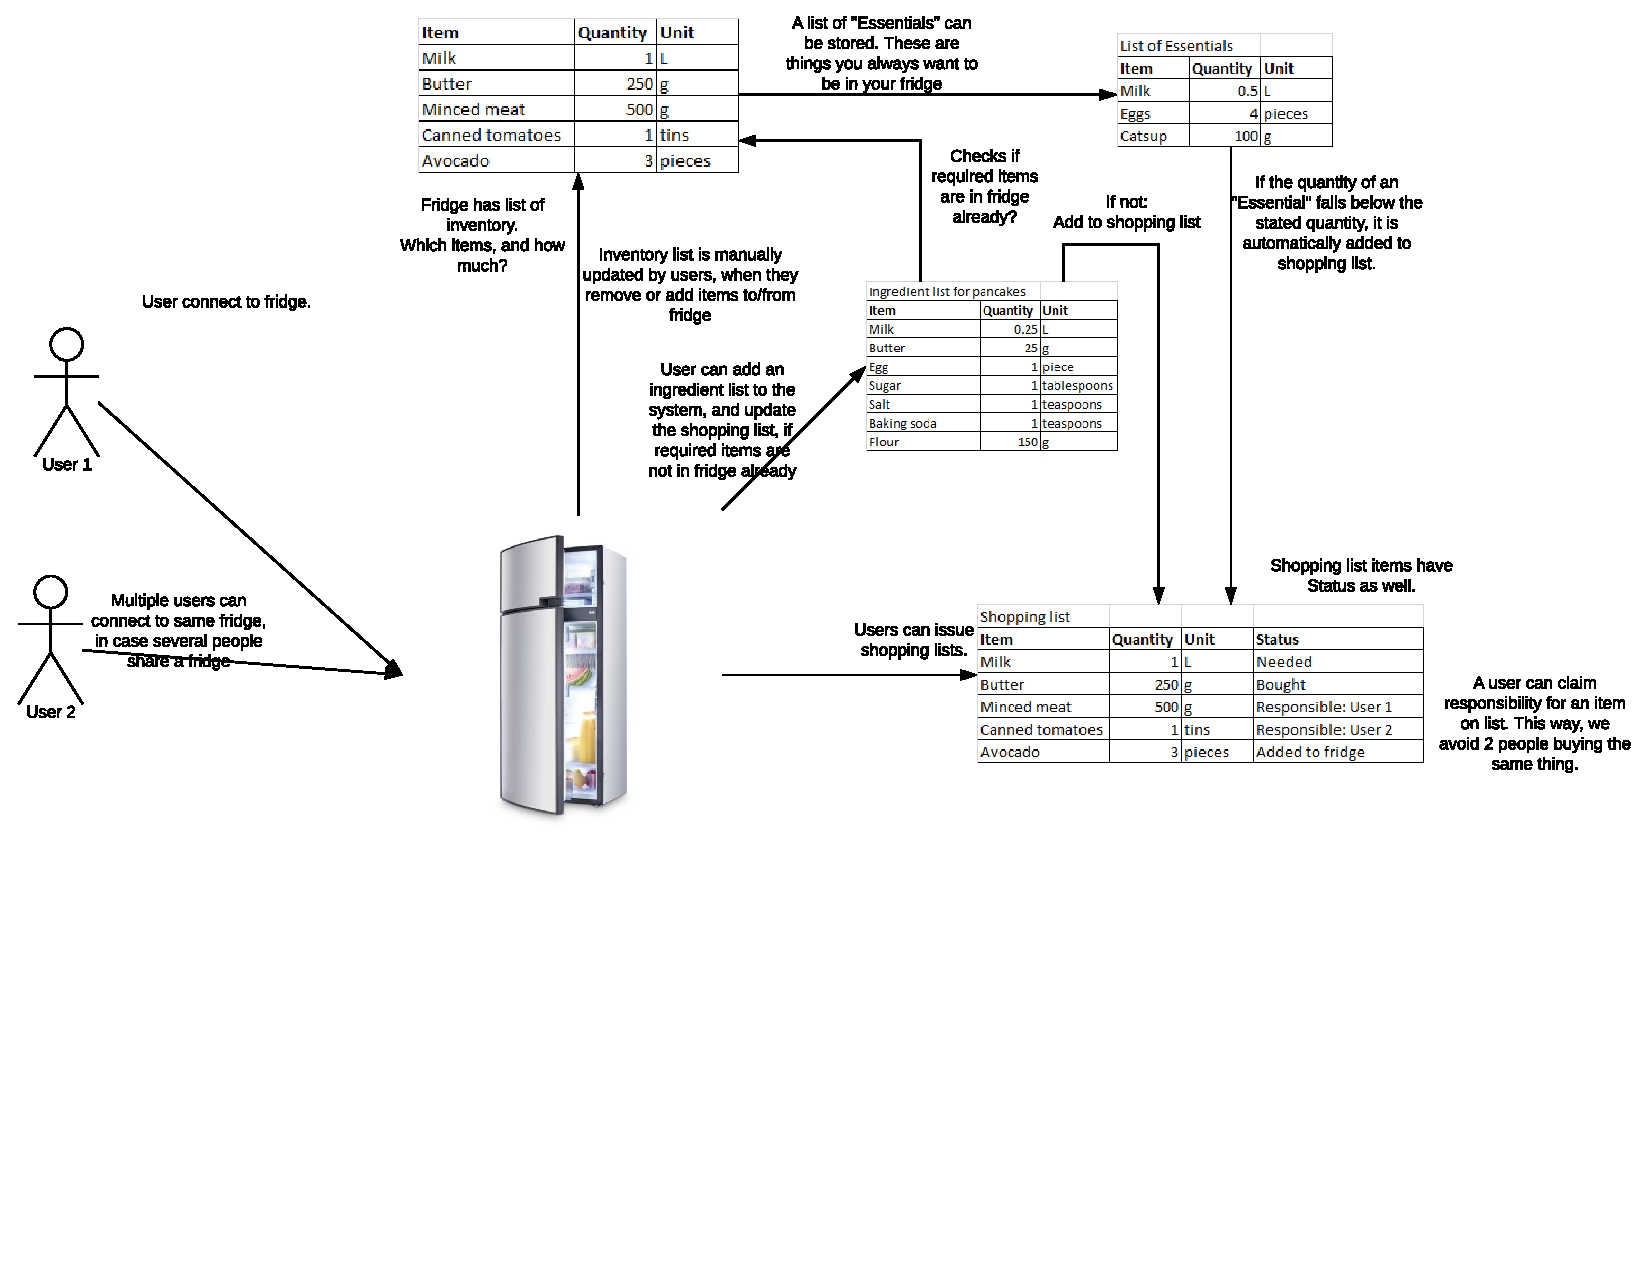
\includegraphics[width=180mm]{Img/Fridge_rich_picture.pdf}
	\caption{Rich picture of Fridge-i-nator}
	% \floatfoot{Source: (Citation command)}
	\label{fig:RichPic}
\end{figure}

\subsection{User stories}

\textbf{CONNECTION}\\
As a user, I can connect to a create a new fridge, so that i can acces connect to it.

As a user, I can connect to a fridge, so that I can access information about it.

As a user, I can add other people to a fridge I am connected to, so that they can access information about it.

As a user, I can leave a fridge, so that I cannot acces information about it anymore.
\newline
\newline
\textbf{INVENTORY}
As a user, I can acces an inventory list of items which the fridges contain, so all users connected to the fridge can keep track of what is in the fridge.

As a user, I can add items to the inventory list, so that all connected users may know that the item is in the fridge.
\newline
\newline
\textbf{SHOPPING LIST}
As a user, I can acces a shopping list of items, so all users connected to the fridge can keep track of what needs to be bought for the fridge.

As a user, I can add items to the shopping list, so that all connected users may know that the item needs to be bought.
\newline
\newline
\textbf{ESSENTIALS LIST}
As a user, I can acces a list of essential items with a minimum quantity of each item, so when the quantity of at specific item comes below the minimum quantity fridge-i-nator automatically adds the item to the shopping list.

As a user, I can add items to the lsit of essential items, so that all the system automatically will add the item to the shopping list, if the quantity of the item falls below a specifiec quantity.
\newline
\newline
\textbf{INGREDIENT LIST}
As a user, I can add an ingredient list of items, so that the system will add missing items to the shopping list.
\newline
\newline
\textbf{USING THE SHOPPIN/INVENTORY LIST}
As a user, I can claim responsibility of an item on the shopping list, so that other useres will be notified about who has taken responsibility of the given item to avoid double shopping.

As a user, I can move an item from the shopping list to the inventory list, so that all users connected to the fridge will know that the item has been bought.


\subsection{Early design}

\begin{figure}[H]
	\centering
	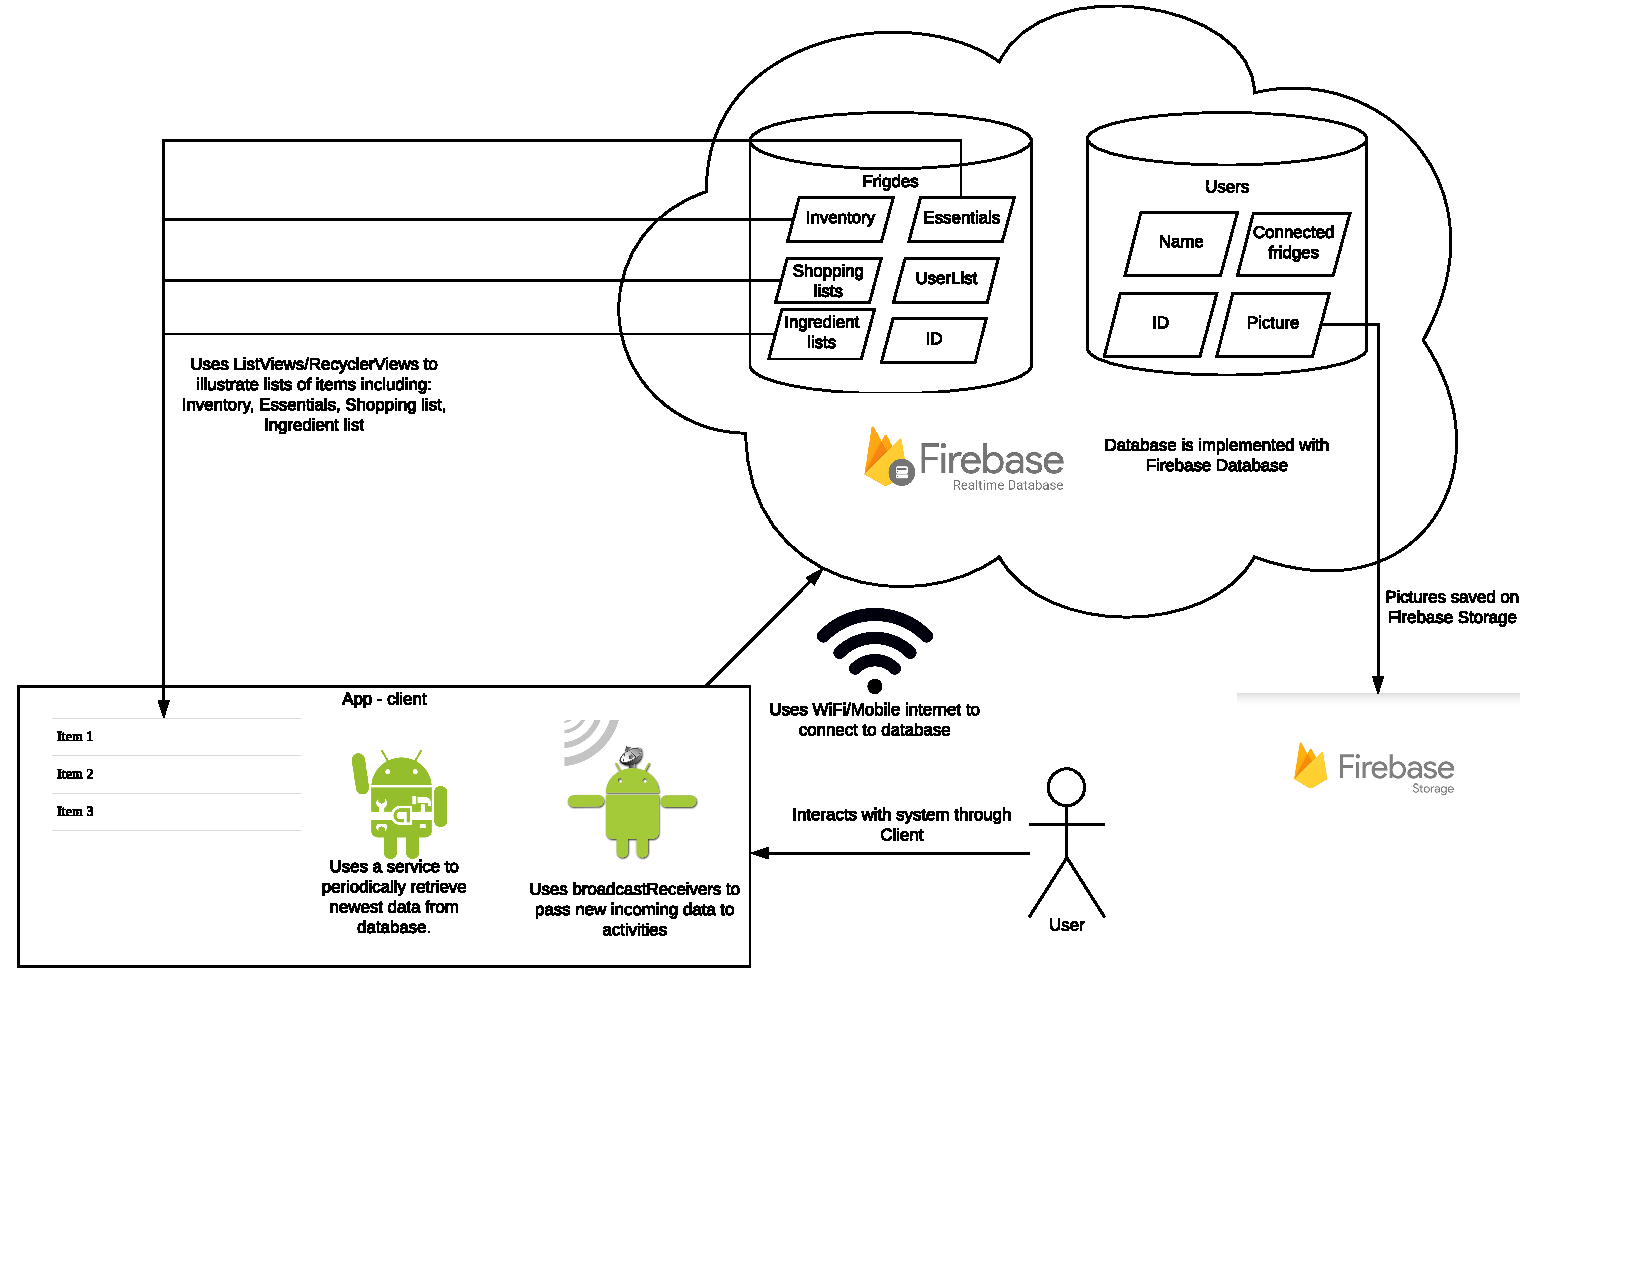
\includegraphics[width=180mm]{Img/Fridge_some_diagram.pdf}
	\caption{Early design diagram of Fridge-i-nator}
	% \floatfoot{Source: (Citation command)}
	\label{fig:Design diagram}
\end{figure}

\subsection{Risks}

- Not able to deliver a working app at deadline
\newline
- Working with firebase without any prior experience

\end{document}